% !TeX encoding = UTF-8
\chapter{Task 3: Data Pre-processing}\label{chap:task3_preprocessing}

The task asks us to analyze the labels, handle infinite and NaN values, scale the features with min-max scaling and select the 20 best features with \texttt{SelectKBest}. We implemented this in Python 3.12 with pandas and scikit-learn~\cite{pedregosa2011sklearn} (modules \texttt{data.py} and \texttt{features.py}, script \texttt{task3\_preprocess.py}). The steps are, in this order:

\begin{enumerate}\setlength\itemsep{0pt}
	\item \textbf{Load and analyze labels.} 65 of the 79 column names carry stray leading spaces and are stripped. The labels are normalized (whitespace collapsed, validated against the two expected classes). For this file this step changes nothing, because the labels are already clean.
	\item \textbf{Drop the duplicate column.} \texttt{Fwd Header Length} appears twice in the header, a known artifact of the CICFlowMeter export. We drop the second copy.
	\item \textbf{Infinity and NaN.} We replace $\pm\infty$ by NaN and \emph{drop} the affected rows. Only 34 rows are affected, 32 BENIGN and 2 DDoS, so dropping loses almost no information and introduces no artificial values. The infinite and NaN values occur only in \texttt{Flow Bytes/s} and \texttt{Flow Packets/s}: CICFlowMeter divides by the flow duration, which is 0 for some flows (a positive byte count divided by 0 gives $\infty$, 0/0 gives NaN).
	\item \textbf{Duplicate rows.} We remove exact duplicates before splitting. Otherwise identical rows land in both train and test sets and inflate the test scores.
	\item \textbf{Constant columns.} They carry no information and trigger warnings in \texttt{SelectKBest}.
	\item \textbf{Identical columns.} Columns equal to an earlier one (tolerance $10^{-6}$) are removed, so that the 20 selected features are distinct. The tolerance is needed for one pair, \texttt{Bwd Packet Length Mean} and \texttt{Avg Bwd Segment Size}: they are the same quantity but differ in 2 rows by at most $10^{-6}$ because of CSV rounding.
	\item \textbf{Train/test split.} A stratified 70/30 split on the label with \texttt{random\_state=42}, done \emph{before} anything is fitted.
	\item \textbf{Min-max scaling.} \texttt{MinMaxScaler(clip=True)} maps each feature to $[0,1]$. It is fitted on the training set only, so no test statistics leak into training, and \texttt{clip=True} keeps unseen values, such as live traffic later, inside $[0,1]$.
	\item \textbf{Feature selection.} \texttt{SelectKBest(chi2, k=20)} on the scaled training set. We scale first because $\chi^2$ requires non-negative input, and the raw data contains negative values: \texttt{Init\_Win\_bytes\_*} is $-1$ when no window was observed, and a few durations are negative.
\end{enumerate}

The column-level steps 5 and 6 use feature values only, never labels, so they leak no label information. Listing~\ref{lst:clean} shows the core of steps 2--6 in the code.

% U+FFFD in data.py (normalize_labels) would otherwise leak into the listing (listings/LuaTeX quirk)
{\catcode"FFFD=9 \lstinputlisting[style=py,float=htbp,linerange={113-114,118-121,134-136,141-143,148-150,155-157},caption={Core cleaning steps of \texttt{clean()} in \texttt{src/ddosids/data.py} (steps 2--6; logging calls omitted)},label={lst:clean}]{../src/ddosids/data.py}}

\section{Results}\label{sec:t3-results}

\ssfig[0.45\linewidth]{SS27}{Raw label summary as printed by the pre-processing script: 97,718 BENIGN and 128,027 DDoS flows (cf.\ Table~\ref{tab:t2labels}).}{fig:ss27}

Table~\ref{tab:t3cleaning} lists the cleaning steps with their effect (Figure~\ref{fig:ss28} shows the script log), and Table~\ref{tab:t3removed} the removed columns. The raw file has 2,633 duplicate rows, but 4 of them contain infinite or NaN values and are already gone after step 3, so step 4 drops 2,629 (2,618 BENIGN, 11 DDoS). The six bulk-transfer features are always 0 in this CICFlowMeter version. \texttt{Fwd PSH Flags} is identical to \texttt{SYN Flag Count}, although PSH and SYN are different TCP flags. This points to a feature-extraction problem in the CICFlowMeter version used for CIC-IDS2017, in line with the literature~\cite{engelen2021troubleshooting}.

\begin{table}[ht]
	\centering\small
	% AUTO-GENERATED by scripts/make_report_tables.py from outputs/task3/cleaning_report.json -- do not edit
\begin{tabularx}{\linewidth}{rlrrX}
\toprule
\# & Step & Rows & Cols & Detail \\
\midrule
1 & Drop duplicate header column & 225\,745$\to$225\,745 & 79$\to$78 & $-$1 column (\texttt{Fwd Header Length.1}) \\
2 & Replace $\pm\infty$ by NaN & 225\,745$\to$225\,745 & 78$\to$78 & inf: \texttt{Flow Bytes/s} 30, \texttt{Flow Packets/s} 34; NaN: \texttt{Flow Bytes/s} 4 \\
3 & Drop NaN rows & 225\,745$\to$225\,711 & 78$\to$78 & $-$34 rows (32 BENIGN, 2 DDoS) \\
4 & Drop duplicate rows & 225\,711$\to$223\,082 & 78$\to$78 & $-$2\,629 rows (2\,618 BENIGN, 11 DDoS) \\
5 & Drop constant columns & 223\,082$\to$223\,082 & 78$\to$68 & $-$10 columns \\
6 & Drop identical columns & 223\,082$\to$223\,082 & 68$\to$60 & $-$8 columns \\
\midrule
 & \textbf{Result} & \textbf{223\,082} &  & \textbf{223\,082 rows $\times$ 59 features} \\
\bottomrule
\end{tabularx}

	\caption{Cleaning steps. The column counts include the \texttt{Label} column, so the 60 remaining columns are 59 features plus \texttt{Label}. Loading and label normalization happen before step 1.}
	\label{tab:t3cleaning}
\end{table}

\ssfig{SS28}{Cleaning steps as logged by the pre-processing script, ending with \enquote{Final: 223082 rows x 59 features} (cf.\ Table~\ref{tab:t3cleaning}).}{fig:ss28}

\begin{table}[ht]
	\centering\small
	% AUTO-GENERATED by scripts/make_report_tables.py from outputs/task3/cleaning_report.json -- do not edit
\begin{tabularx}{\linewidth}{lX}
\toprule
Kind & Columns \\
\midrule
Constant (10) & \texttt{Bwd PSH Flags}, \texttt{Fwd URG Flags}, \texttt{Bwd URG Flags}, \texttt{CWE Flag Count}, \texttt{Fwd Avg Bytes/Bulk}, \texttt{Fwd Avg Packets/Bulk}, \texttt{Fwd Avg Bulk Rate}, \texttt{Bwd Avg Bytes/Bulk}, \texttt{Bwd Avg Packets/Bulk}, \texttt{Bwd Avg Bulk Rate} \\
\midrule
Identical & \texttt{Fwd PSH Flags} $\to$ \texttt{SYN Flag Count} (dropped) \\
Identical & \texttt{RST Flag Count} $\to$ \texttt{ECE Flag Count} (dropped) \\
Identical & \texttt{Fwd Packet Length Mean} $\to$ \texttt{Avg Fwd Segment Size} (dropped) \\
Identical & \texttt{Bwd Packet Length Mean} $\to$ \texttt{Avg Bwd Segment Size} (dropped) \\
Identical & \texttt{Total Fwd Packets} $\to$ \texttt{Subflow Fwd Packets} (dropped) \\
Identical & \texttt{Total Length of Fwd Packets} $\to$ \texttt{Subflow Fwd Bytes} (dropped) \\
Identical & \texttt{Total Backward Packets} $\to$ \texttt{Subflow Bwd Packets} (dropped) \\
Identical & \texttt{Total Length of Bwd Packets} $\to$ \texttt{Subflow Bwd Bytes} (dropped) \\
\bottomrule
\end{tabularx}

	\caption{Removed columns. For identical pairs, the first column is kept and the second one dropped.}
	\label{tab:t3removed}
\end{table}

After cleaning, 223,082 flows with 59 features remain: 95,068 BENIGN and 128,014 DDoS (Table~\ref{tab:t2labels}), so DDoS stays the majority class. Table~\ref{tab:t3split} shows the split: the test set contains 66,925 flows, of which 38,404 are DDoS.

\begin{table}[ht]
	\centering\small
	% AUTO-GENERATED by scripts/make_report_tables.py from artifacts/clean.parquet, artifacts/split_indices.json -- do not edit
\begin{tabular}{lrr}
\toprule
Label & Train (70\,\%) & Test (30\,\%) \\
\midrule
BENIGN & 66\,547 & 28\,521 \\
DDoS & 89\,610 & 38\,404 \\
\midrule
\textbf{Total} & \textbf{156\,157} & \textbf{66\,925} \\
\bottomrule
\end{tabular}

	\caption{Stratified 70/30 split (\texttt{random\_state=42}).}
	\label{tab:t3split}
\end{table}

\ssfig[0.5\linewidth]{SS29}{Final label summary after cleaning and the class counts of the stratified 70/30 split (cf.\ Tables~\ref{tab:t2labels} and~\ref{tab:t3split}).}{fig:ss29}

On the training set, each of the six example features in Table~\ref{tab:t3scaling} has a scaled minimum of 0 and a maximum of 1. The durations and inter-arrival times, with maxima near the 120\,s timeout, are heavy-tailed and keep modest means after scaling.

\begin{table}[ht]
	\centering\small
	% AUTO-GENERATED by scripts/make_report_tables.py from outputs/task3/describe_train_{before,after}_scaling.csv -- do not edit
\begin{tabular}{lrrrrrr}
\toprule
 & \multicolumn{3}{c}{Before scaling} & \multicolumn{3}{c}{After scaling} \\
\cmidrule(lr){2-4}\cmidrule(lr){5-7}
Feature & Min & Max & Mean & Min & Max & Mean \\
\midrule
\texttt{Init\_Win\_bytes\_backward} & $-$1 & 65\,535 & 616.5311 & 0 & 1 & 0.0094 \\
\texttt{Init\_Win\_bytes\_forward} & $-$1 & 65\,535 & 4\,289 & 0 & 1 & 0.0655 \\
\texttt{Destination Port} & 0 & 65\,532 & 9\,036 & 0 & 1 & 0.1379 \\
\texttt{Flow Duration} & $-$1 & 119\,999\,937 & 16\,472\,365 & 0 & 1 & 0.1373 \\
\texttt{Bwd IAT Total} & 0 & 120\,000\,000 & 6\,626\,749 & 0 & 1 & 0.0552 \\
\texttt{PSH Flag Count} & 0 & 1 & 0.3556 & 0 & 1 & 0.3556 \\
\bottomrule
\end{tabular}

	\caption{Six example features of the training set before and after min-max scaling.}
	\label{tab:t3scaling}
\end{table}

\texttt{URG Flag Count} and \texttt{Destination Port} lead the 20 selected features (Table~\ref{tab:t3top20}; scores in Figure~\ref{fig:fsbin}, script output in Figure~\ref{fig:ss30}) with scores above 28,000 each, and the scores fall steadily down the ranking.

\begin{table}[ht]
	\centering\small
	% AUTO-GENERATED by scripts/make_report_tables.py from outputs/task3/feature_scores_binary.csv -- do not edit
\begin{tabular}{rlr}
\toprule
Rank & Binary feature & $\chi^2$ \\
\midrule
1 & \texttt{URG Flag Count} & 30058.11 \\
2 & \texttt{Destination Port} & 28476.04 \\
3 & \texttt{Bwd Packet Length Max} & 22196.57 \\
4 & \texttt{Bwd Packet Length Std} & 15201.54 \\
5 & \texttt{Bwd Packet Length Mean} & 13631.13 \\
6 & \texttt{Bwd IAT Total} & 10104.71 \\
7 & \texttt{Max Packet Length} & 9940.91 \\
8 & \texttt{Packet Length Mean} & 9735.77 \\
9 & \texttt{Fwd Packet Length Max} & 9338.26 \\
10 & \texttt{Packet Length Std} & 9282.63 \\
11 & \texttt{Average Packet Size} & 8361.12 \\
12 & \texttt{Fwd Packet Length Mean} & 8326.59 \\
13 & \texttt{Fwd PSH Flags} & 7104.49 \\
14 & \texttt{Packet Length Variance} & 6816.96 \\
15 & \texttt{Bwd IAT Max} & 6626.18 \\
16 & \texttt{Fwd Packet Length Std} & 6519.34 \\
17 & \texttt{PSH Flag Count} & 5771.95 \\
18 & \texttt{Down/Up Ratio} & 4499.68 \\
19 & \texttt{Fwd Packet Length Min} & 3409.00 \\
20 & \texttt{Bwd IAT Std} & 3351.57 \\
\bottomrule
\end{tabular}

	\caption{The 20 best features by $\chi^2$ score (min-max-scaled training set), binary target.}
	\label{tab:t3top20}
\end{table}

\ssfig[0.5\linewidth]{SS30}{The top features by $\chi^2$ as printed by the pre-processing script (binary target, ranks 1--20; cf.\ Table~\ref{tab:t3top20}).}{fig:ss30}

\begin{figure}[ht]
	\centering
	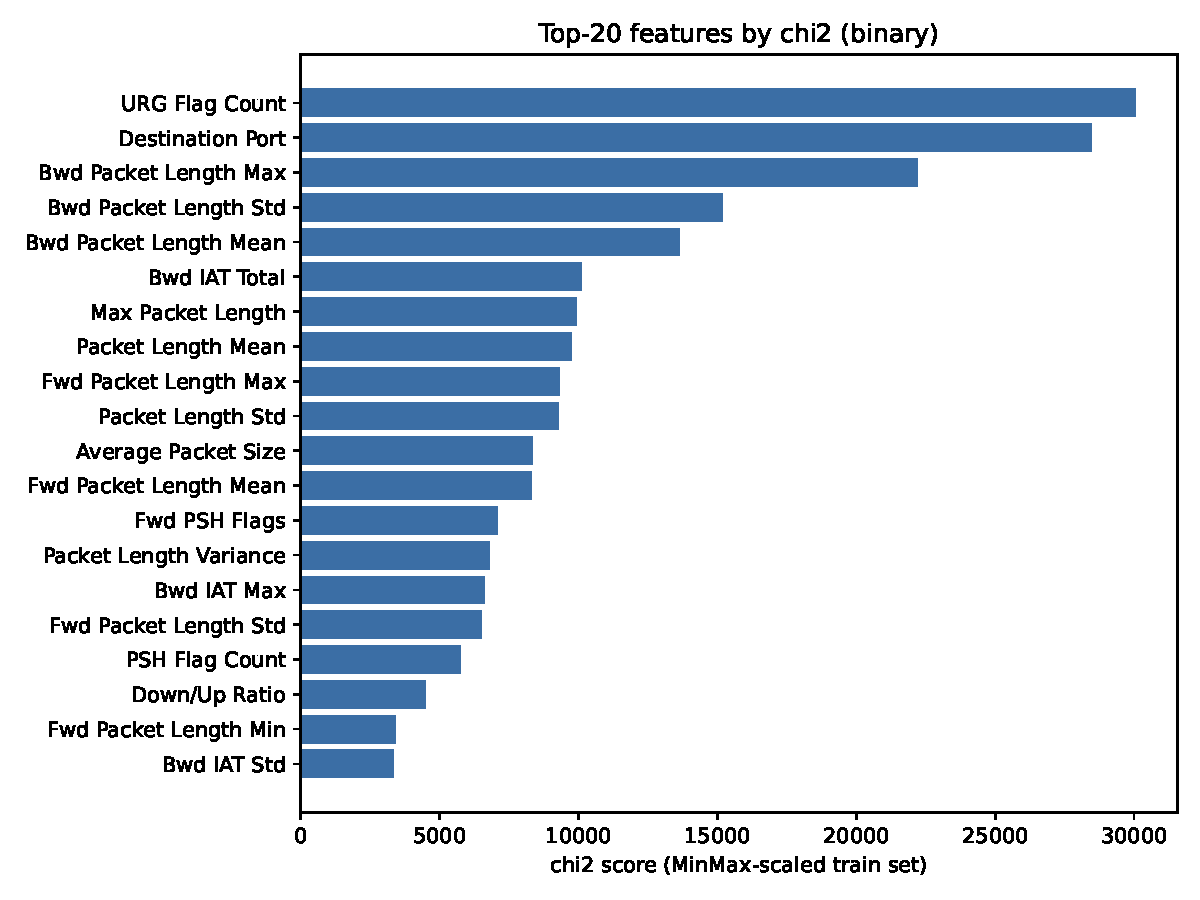
\includegraphics[width=0.75\linewidth]{feature_scores_binary.pdf}
	\caption{Top-20 flow features by $\chi^2$ score for binary classification (BENIGN vs.\ DDoS), computed on the min-max-scaled training set.}
	\label{fig:fsbin}
\end{figure}


\section{Interpretation}\label{sec:t3-interp}

The top-20 list is dominated by packet-size features: twelve of the 20 features describe packet lengths (forward and backward length statistics, the overall maximum, mean, standard deviation and variance, and the average packet size). This is plausible for a flooding attack, whose requests are likely more uniform than the mix of benign traffic. Three features are TCP flag counts (\texttt{URG Flag Count}, \texttt{Fwd PSH Flags}, \texttt{PSH Flag Count}), three describe backward inter-arrival times, and \texttt{Down/Up Ratio} captures the traffic asymmetry. \texttt{Destination Port} ranks second, and virtually all DDoS flows target port 80, so a model can learn ``port 80 is suspicious'' instead of the attack behavior. We expect such testbed-specific features to generalize poorly to other networks. The $\chi^2$ test on min-max-scaled continuous data is also only a heuristic: it treats scaled values like frequencies, and heavy-tailed features are squeezed towards 0, which lowers their scores. The ranking therefore depends on the scaling.

\FloatBarrier
